\section{Análise preliminar}

Utilizarei a biblioteca \emph{sympy} em \emph{Python} para fazer a análise simbólica e numérica do circuito antes de montá-lo fisicamente.

Após terminar as análises compararei os resultados obtidos nas análises numéricas e em laboratório para verificar sua coerência.

Utilizaremos valores de $n = [2,2]$ para o nosso projeto. Isso vem de operações feitas com os CPFs da dupla.

E teremos todas entradas com corrente limitada a $0.75mA$, e uma tensão máxima de $5V$.

\subsection{O circuito}

\begin{figure}[h]
    \centering
    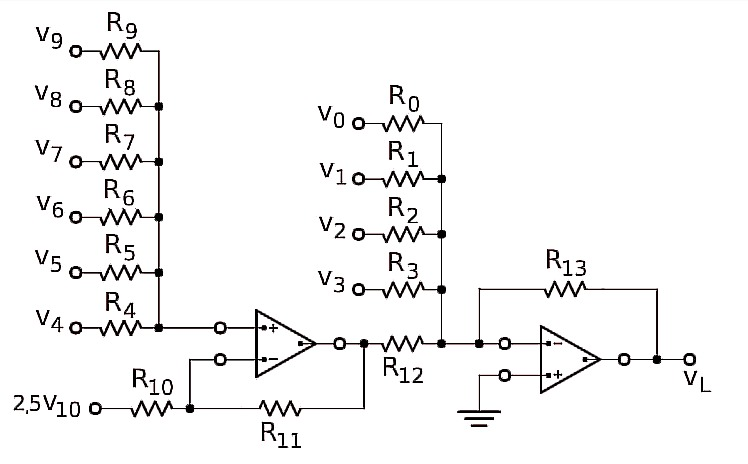
\includegraphics[width=0.6\columnwidth]{images/circuito.jpeg}
    \caption{Planta esquemática do DAC de 11-bits.}
\end{figure}


\newpage
\subsection{Análise simbólica}

Podemos realizar a análise do circuito utilizando análise nodal e princípio da superposição. Com isso, obtém-se a seguinte equação que rege a saída $V_L$ do circuito.


\begin{equation}
    \label{eq:VL}
    V_L = - \left( R_{13} \sum_{i=0}^{3} \frac{V_i}{R_i} + \frac{R_{13}}{R_{12}} \left( 1 + \frac{R_{11}}{R_{10} }\right)  R_{eq} \sum_{i=4}^{9} \frac{V_i}{R_i}- \frac{R_{11}R_{13}}{R_{10} R_{12}} 2.5 V_{10} \right)
\end{equation}

Comparamos este $V_L$ com uma saída \emph{M} do DAC.

\begin{equation}
    \label{eq:M}
    M = r\left(\sum_{i=0}^{n-1} d_i 2^{i} - d_n 2^n\right)
\end{equation}

\subsubsection{Resolução}

Onde $r$ é a resolução do DAC, $d_i$ é o valor do bit $i$ e $n$ é o número de bits do DAC.

Para o nosso projeto, escolheremos uma tensão máxima de $V_L = M = 7V$.

Com as equações \ref{eq:VL} e \ref{eq:M}, analisaremos o comportamento das equações para diferentes configurações de bits $d_i$ ligados.

Para obter a resolução $r$, analisamos o valor máximo possível de $2^n$ para 10 bits, e consideraremos que tanto o valor máximo positivo quanto negativo serão os mesmos, que serão $1024$.

Então, com \ref{eq:M}, tem-se:

\begin{equation}
    r = \frac{7}{2^{10}}
\end{equation}

\subsubsection{Resistores}

Analisaremos o comportamento de \ref{eq:VL} e \ref{eq:M} para diferentes configurações de bits $d_i$ ligados.

Como queremos ter uma limitação de corrente de $0.75mA$ em todas as entradas, podemos aplicar a lei de Ohm com apenas o $d_3$ ligado e encontrar o valor de $R_3$.


\begin{equation}
    \begin{aligned}
         & V_3 = V_m d_3 = I R_3                               \\
         & I = 0.75mA > \frac{V_m}{R_3}                        \\
         & R_3 > \frac{5V}{ 0.75mA} = \frac{20}{3} k \varOmega
    \end{aligned}
\end{equation}

No caso, escolhemos $R_3 = 100k \Omega$, o que atende à condição de limitação de corrente.

Para manter os pesos vistos na equação $eq:M$ nos resistores deste amplificador operacional, fazemos a mesma lógica para $R_2, R_1 e R_0$, ou seja, dobramos o valor de cada um deles considerando o anterior, e obtemos:

\begin{equation}
    \begin{aligned}
         & R_2 = 2 R_3 = 200k \varOmega \\
         & R_1 = 2 R_2 = 400k \varOmega \\
         & R_0 = 2 R_1 = 800k \varOmega
    \end{aligned}
\end{equation}

Com estes quatro determinados, agora buscamos o $R_{13}$, vemos que em \ref{eq:VL}, se zerarmos todas as entradas, exceto uma entrada entre $0$ e $3$, conseguimos novamente utilizar a relação $V_L = M$ e obter o $R_{13}$.

\begin{equation}
    \begin{aligned}
         & \frac{R_{13} V_m }{R_i r} = 2^i \\
         & R_{13} = 1093.75 \varOmega
    \end{aligned}
\end{equation}

Agora fazemos as restrições de corrente para as entradas de $4$ a $9$. Para isso, precisamos saber a tensão mínima possível para $V_a$. Isolamos o $V_a$ pela resolução das equações da análise nodal no \emph{Sympy}, que se encontra no apêndice. E obtemos:

\begin{equation}
    V_a = \sum_{i=4}^{9} \frac{V_i R_eq}{R_i}
\end{equation}

Os três termos da equação nunca serão negativos, e o único que pode ser zero é o $V_i$, logo, o valor mínimo de $V_a$ é $0V$.

Daqui podemos fazer a análise com $d_i$ com apenas um ligado entre $4$ e $9$ e obter os resistores $R_4$ a $R_9$.

Com a mesma lógica que obtemos resistores de $0$ a $3$, vamos encontrar o $R_9$ que é o mais significativo, e a partir dele, obteremos os outros $5$.

\begin{equation}
    R_9 > \frac{20}{3} \varOmega
\end{equation}

Nós escolhemos um valor de $R_9 = 22k \Omega$ que atende à restrição.

Para calcular o $R_{10}$, $R_{11}$ e $R_{12}$, utilizaremos as seguintes relações:

\begin{equation}
    \label{eq:XY}
    \begin{aligned}
         & X = \frac{R_{11}}{R_{10}} \\
         & Y = \frac{R_{13}}{R_{12}} \\
    \end{aligned}
\end{equation}

Então, desligando todas as entradas, exceto $d_{10}$, a partir de \ref{eq:VL} e \ref{eq:M}, e com as substituições \ref{eq:XY}, tem-se:

\begin{equation}
    \begin{aligned}
        X Y = 2.5 V_0 = 2.5 V_m d_{10} \\
        X Y = \frac{7}{12.5} = 0.56
    \end{aligned}
\end{equation}

Nas equações \ref{eq:VL}, \ref{eq:M} e fazendo as substituições \ref{eq:XY}, fazendo apenas a entrada $d_{9}$ estar ligada, e atentando-se que o $R_{eq}$ é a resistência equivalente entre o $R_4$ até o $R_9$ e vale $11175\Omega$, tem-se:

\begin{equation}
    \begin{aligned}
         & Y ( 1 + X ) R_{eq} \frac{V_9}{R_9} = \frac{7}{2} \\
         & Y ( 1 + X ) = 1.38                               \\
    \end{aligned}
\end{equation}

Resolvendo o sistema

\begin{equation}
    \begin{aligned}
         & Y ( 1 + X ) = 1.38          \\
         & X Y = \frac{7}{12.5} = 0.56 \\
    \end{aligned}
\end{equation}

Obtém-se: $X = 0.684$ e $Y = 0.818$.

Convertendo de volta o $X$ e $Y$, tem-se:

\begin{equation}
    \begin{aligned}
         & \frac{R_{11}}{R_{10}} = 0.684 \\
         & \frac{R_{13}}{R_{12}} = 0.818 \\
    \end{aligned}
\end{equation}

Como já havíamos obtido o $R_{13}$ previamente, obtemos o valor exato do $R_{12}$, que é $R_{12} = 1337 \varOmega$.

Já o $R_{11}$ e $R_{10}$ têm apenas uma proporção entre os dois. Então, escolhemos valores comerciais de $R_{11} = 15k \Omega$ e $R_{12} = 22k \Omega$.

E com isso, determina-se os $15$ resistores do projeto.

